\documentclass[10pt]{standalone}
\usepackage{amsmath}
\usepackage{pgf,tikz}
\usepackage{mathrsfs}
\usetikzlibrary{arrows}
\pagestyle{empty}
\begin{document}
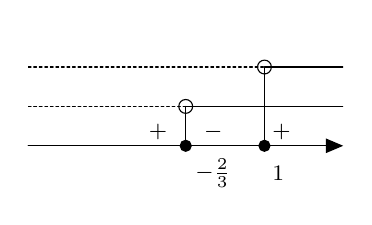
\begin{tikzpicture}[line cap=round,line join=round,>=triangle 45,x=1.0cm,y=1.0cm]
\draw[->] (-2.,0.) -- (2.,0.);
\draw[color=black] (0pt,-10pt) node[right] {\footnotesize $-\frac{2}{3}$};
\clip(-2.,-0.5) rectangle (2.,1.5);
\draw (0.,0.)-- (0.,0.5);
\draw (0.,0.5)-- (2.,0.5);
\draw [dash pattern=on 1pt off 1pt] (-2.,0.5)-- (0.,0.5);
\draw  (1.,1.)-- (1.,0.);
\draw  (2.,1.)-- (1.,1.);
\draw [dash pattern=on 1pt off 1pt] (-2.,1.)-- (1.,1.);
\begin{scriptsize}
\draw [fill=black] (0.,0.) circle (2.0pt);
\draw  (0.,0.5) circle (2.5pt);
\draw (1,-10pt) node[right] {\footnotesize $1$};
\draw  (1.,1.) circle (2.5pt);
\draw [fill=black] (1.,0.) circle (2.0pt);
\draw[color=black] (-10pt,5pt) node {\footnotesize $+$};
\draw[color=black] (10pt,5pt) node {\footnotesize $-$};
\draw (1,5pt) node[right] {\footnotesize $+$};
\end{scriptsize}
\end{tikzpicture}
\end{document}